% --------------------------------------------------------------------------------

\begin{exercise}[272]

Betrachten Sie die folgenden Eigenschaften, die eine Menge $A$ haben kann:

\begin{enumerate}[label = \alph*.]
  \item Es gibt eine injektive Abbildung von $\omega$ nach $A$. (\enquote{$\omega \leq A$})
  \item Es gibt eine fast injektive Abbildung von $\omega$ nach $A$.
  (\enquote{fast injektiv} bedeutet, dass das Urbild jedes Bildpunktes endlich ist.)
  \item Es gibt eine injektive, aber nicht surjektive Abbildung von $A$ nach $A$.
  \item Es gibt eine fast injektive, aber nicht surjektive Abbildung von $A$ nach $A$.
  \item Für ein (alle) $x \notin A$ gibt es eine Bijektion von $A$ nach $A \cup \Bbraces{x}$.
  (\enquote{$A = A + 1$})
  \item Es gibt eine surjektive, aber nicht injektive Abbildung von $A$ nach $A$.
  \item Es gibt eine surjektive Abbildung von $A$ auf $\omega$. (\enquote{$\omega \leq^* A$})
  \item Es gibt eine surjektive, fast injektive Abbildung von $A$ auf $\omega$.
  \item Es gibt eine injektive Abbildung von $\omega$ nach $P(A)$. (\enquote{$\omega \leq P(A)$})
  \item Es gibt eine injektive Abbildung von $\omega$ in die endlichen Teilmengen von $A$. (\enquote{$\omega \leq P_\mathrm{fin}(A)$})
  \item Es gibt eine surjektive Abbildung von den endlichen Teilmengen von $A$ auf $\omega$.
  \item $A$ ist unendlich: \enquote{$|A| = \infty$}
  \item Es gibt eine nichtleere Teilmenge von $\mathfrak{P}(A)$ ohne (bez. $\subseteq$) maximales Element.
\end{enumerate}

Geben Sie möglichst viele nichttriviale Implikationen zwischen diesen Aussagen an, die sich in ZF (also ohne Auswahlaxiom) beweisen lassen.

\end{exercise}

% --------------------------------------------------------------------------------

\begin{solution}

\phantom{}

\begin{tikzpicture}[
	> = stealth, % arrow head style
	shorten > = 1pt, % don't touch arrow head to node
	auto,
	node distance = 3cm, % distance between nodes
	semithick % line style
	]
	
	\tikzstyle{every state}=[
	draw = black,
	thick,
	fill = white,
	minimum size = 4mm
	]
	
	\node[state] (a) {$a$};
	\node[state] (b) [above of=a] {$b$};
	\node[state] (c) [right of=a] {$c$};
	\node[state] (f) [below right of=a] {$f$};
	\node[state] (h) [below of=a] {$h$};
	\node[state] (d) [right of=c] {$d$};
	\node[state] (e) [below right of=c] {$e$};
	\node[state] (g) [below left of=a] {$g$};
	\node[state] (j) [above left of=a] {$j$};
	\node[state] (i) [left of=j] {$i$};
	\node[state] (k) [left of=a] {$k$};
	\node[state] (l) [above right of=a] {$l$};
	\node[state] (m) [right of=l] {$m$};

	
	\path[->] (a) edge [bend left] node {} (b);
	\path[->] (b) edge [bend left] node {} (a);
	\path[->] (c) edge [bend left] node {} (a);
	\path[->] (a) edge node {} (c);
	\path[->] (a) edge node {} (f);
	\path[->] (a) edge [red] node {} (h);
	\path[->] (c) edge node {} (d);
	\path[->] (e) edge node {} (c);
	\path[->] (e) edge [dotted] node {} (f);
	\path[->] (a) edge node {} (g);
	\path[->] (a) edge node {} (j);
	\path[->] (j) edge node {} (i);
	\path[->] (h) edge node {} (g);
	\path[->] (j) edge node {} (k);
	\path[->] (g) edge node {} (k);
	\path[->] (l) edge node {} (m);
	\path[->] (a) edge node {} (l);
	\path[->] (l) edge [dashed, bend left] node {} (a);
\end{tikzpicture}

Hier einige Inklusionen, im Bild oben als durchgehende schwarze Pfeile eingezeichnet.

\begin{enumerate}[label = \texttt{ad}]
	\item \enquote{a. $\implies$ b.}:
	
	Klar!
	
	\item \enquote{b. $\implies$ a.}:
	
	\begin{enumerate}[label = \arabic*.]
		
		\item Lösung:
		
		Sei $f: \omega \to A$ fast injektiv, d.h.
		
		\begin{align*}
		\Forall x \in f[\omega]:
		|f^{-1}[\Bbraces{x}]| < \infty.
		\end{align*}
		
		Wir fassen $\omega$ und $A$ als Algebren mit leerem Typ auf.
		Auf diese können wir also den Homomorphiesatz anwenden und bekommen eine Abbildung $g$.
		
		\textbf{Achtung!}
		Möglicherweise braucht der Homomorphiesatz das Auswahlaxiom?
		Anstatt einen beliebigen Repräsentanten $u$ von $U$ zu wählen, kann man in unserem Fall den kleinsten $u := \min U$ (von endlich vielen) wählen, um $g(U) := f(u)$ zu definieren.
		Wir haben es schließlich mit Schuhen und nicht mit Socken zu tun!
		
		\phantom{}
		
		\begin{tcolorbox}[standard jigsaw, opacityback = 0]
			\centering
			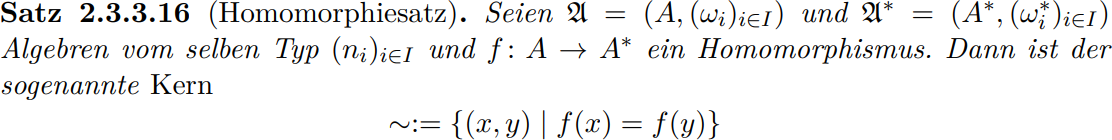
\includegraphics
			[width = 0.75 \textwidth]
			{Alg/Alg - Satz 2.3.3.16.1 (Homomorphiesatz).png} \\
			\vspace{0.25 cm}
			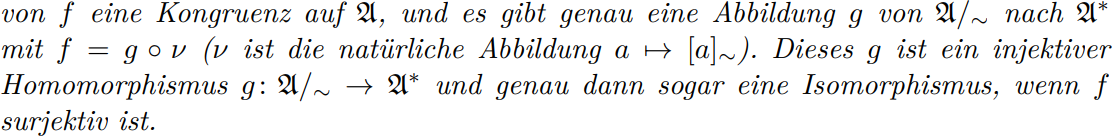
\includegraphics
			[width = 0.75 \textwidth]
			{Alg/Alg - Satz 2.3.3.16.2 (Homomorphiesatz).png} \\
			\vspace{0.25 cm}
			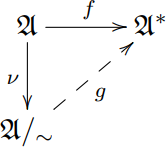
\includegraphics
			[width = 0.15 \textwidth]
			{Alg/Alg - Satz 2.3.3.16.3 (Homomorphiesatz).png}
		\end{tcolorbox}
		
		\phantom{}
		
		Seien die (unendlich vielen!) Urbilder gemäß ihrem Minimum, vermöge $h$ (strikt monoton steigend), geordnet, d.h.
		
		\begin{align*}
		h := (U_n)_{n \in \omega}:
		\omega \to \omega / \sim:
		\min U_1 < \min U_2 < \cdots
		\end{align*}
		
		$g \circ h: \omega \to A$ ist, als Verkettung injektiver Funktionen, injektiv.
		
		\item Lösung:
		
		Sei $f: \omega \to A$ fast injektiv. \\
		Definiere die injektive Funktion $f': \omega \to A$ durch
		\begin{align*}
		f'(0) &:= f(0) \\
		f'(n) &:= f(\min\{k \in  \N:  f(k) \notin f[\{0,\dots,n-1\}]\}), \quad n \geq 1.
		\end{align*}
		Da das Urbild jedes Bildpunktes endlich ist, exisitiert dieses Minimum immer.
		
	\end{enumerate}

	\item \enquote{a. $\implies$ c.}: Sei $f: \omega \to A$ injektiv.
	Definiere
	\begin{align*}
	g := \{(f(n),f(n+1)): n \in \omega\} \cup \{(a,a): a \in A \setminus f(\omega)\}
	\end{align*}
	$g$ ist sicher auf ganz $A$ definiert, injektiv und es gilt $f(0) \notin g(A)$.
	
	Diese Implikation wurde auch in Aufgabe 269 gezeigt.
	
	\item \enquote{c. $\implies$ a.}: Siehe letzte Übung Aufgabe 270.
	
	\item \enquote{c. $\implies$ d.}:
	
	Klar.
	
	\item \enquote{e. $\implies$ c.}:
	
	Sei $x \not \in A$ und $f: A \to A \cup \Bbraces{x}$ bijektiv.
	$f^{-1} |_A: A \to A$ ist injektiv, trifft aber nicht $f^{-1}(x)$, ist also nicht surjektiv.
	
	\item \enquote{a. $\implies$ f.}: Sei $f: \omega \to A$ injektiv. Definiere
	
	\begin{align*}
	g := \{(f(n+1),f(n)): n \in \omega\} \cup \{(a,a): a \in A \setminus f(\omega)\}
	\cup \{(f(0),f(0))\}
	\end{align*}
	$g$ ist surjektiv, aber nicht injektiv.
	
	\item \enquote{h. $\implies$ g.}:
	
	Klar!
	
	\item \enquote{a. $\implies$ g.}:
	
	Sei $f: \omega \to A$ injektiv.
	Es gibt folglich also eine (surjektive) Linksinverse $f^{-1}: f[\omega] \to \omega$.
	Wir setzen diese zu einer (surjektiven) Funktion $g: A \to \omega$ beliebig fort.
	
	\item \enquote{g. $\implies$ k.}:
	
	Sei $f: A \to \omega$ surjektiv.
	
	\begin{gather*}
	g:
	P(A) \to \omega:
	M \mapsto \min f[M],
	\quad
	g_\mathrm{fin} := g |_{P_\mathrm{fin}(A)},
	\quad
	g_\mathrm{sing} := g_\mathrm{fin} |_{P_\mathrm{sing}(A)} \cong f \\
	\implies
	\omega
	\supseteq
	g(P(A))
	\supseteq
	g_\mathrm{fin}(P_\mathrm{fin}(A))
	\supseteq
	g_\mathrm{sing}(P_\mathrm{sing}(A))
	=
	f(A)
	=
	\omega
	\end{gather*}
	
	$g$, $g_\mathrm{fin}$, und $g_\mathrm{sing}$ sind also auch allersamt surjektiv.
	
	\item \enquote{a. $\implies$ j.}:
	
	Sei $f: \omega \to A$ injektiv, so auch $g: \omega \to P_\mathrm{fin}(A): n \to \Bbraces{n}$.
	
	\item \enquote{j. $\implies$ i.}:
	
	Klar!
	
	\item \enquote{j. $\implies$ k.}:
	
	Verwende \enquote{a. $\implies$ g.} für $P_\mathrm{fin}(A)$ anstelle von $A$.
	
	\item \enquote{a. $\implies$ l.}:
	
	Wir führen einen Widerspruchsbeweis. Sei also $A$ endlich mit $n \in \omega$ und $f: A \to n$ bijektiv und $g: \omega \to A$ injektiv. Dann ist $h:= g \circ g: \omega \to n$ ebenfalls injektiv. Das kann aber nicht sein, denn wir sehen induktiv, dass
	\begin{align*}
		\forall k \in \omega: \forall \alpha: \omega \to k: \alpha \text{ nicht injektiv. }
	\end{align*}
	Für $k = 0 = \emptyset$ gibt es gar keine Abbildung $\alpha: \omega \to k$, also ist die Aussage klar.
	
	Nehmen wir nun also an, die Aussage gilt bereits für $k \in \omega$. Weiters nehmen wir an, es git eine injektive Funktion $\alpha: \omega \to k + 1$. Wegen der Injektivität gibt es genau ein $l \in \omega$ mit $\alpha(l) = \{k\}$. Nun finden wir die injektive Funktion 
	\begin{align*}
		u: \omega \to \omega: x \mapsto
		\begin{cases}
			x &, \text{falls } x < l \\
			x + 1 &, \text{falls } x \geq l
		\end{cases}.
	\end{align*}
	Nun ist $\beta: \omega \to n: x \mapsto \alpha(u(x))$ eine injektive Funktion. Ein Widerspruch zur Induktionsvoraussetzung. 
	
	\item \enquote{l. $\implies$ m.}:
	
	Sei also $A$ eine undenliche Menge. Definiere
	\begin{align*}
	\mathfrak{M}:=\Bbraces{X \subseteq A \mid X \text{ endlich }}
	\end{align*}
	und sei $X \in \mathfrak{M}$ beliebig. Die Menge $X$ ist endlich, also gibt es ein $n \in \omega$ und eine Bijektion $f:n \to X$. Da $A$ unendlich ist, kann $f:n \to A$ nicht surjektiv sein also gibt es $y \in A \setminus f[n]$. Nun definiere $Z := X \cup \{y\}$ und
	\begin{align*}
	g:n + 1 \to Z: m \mapsto
	\begin{cases}
	y & ,\text{falls } m = n \\
	f(m) & ,\text{sonst }
	\end{cases}.
	\end{align*}
	Wir sehen, dass $g$ bijektiv ist also $Z$ endlich aber $Z \supsetneq X$, also ist $X$ nicht maximal.
\end{enumerate}




Hier Implikationen die sicher nicht gelten, im Bild oben als rote Pfeile eingezeichnet.

\begin{enumerate}[label = \texttt{ad}]
	\item \enquote{a. $\implies$ h.}: Wenn $f: A \to \omega$ eine surjektive und fast injektive Abbildung ist, dann können wir $A$ schreiben als
	\begin{align*}
		A = f^{-1}(\omega) = f^{-1}\pbraces{\bigcup_{n \in \omega} \Bbraces{n}} = \bigcup_{n \in \omega} f^{-1}\pbraces{\{n\}}
	\end{align*}
	und da $f^{-1}\pbraces{{n}}$ für jedes $n$ endlich ist wissen wir, dass $A$ höchstens abzählbar unendlich sein kann. Da wir aber schon überabzählbar unendliche Mengen kennen kann diese Inklusion im Allgemeinen nicht gelten. 
\end{enumerate}


Hier Implikationen, für die man (zumindest laut Skriptum) das Auswahlaxiom braucht. Im Graphen oben sind das die strichlierten Pfeile.
\begin{enumerate}[label = \texttt{ad}]
	\item \enquote{l. $\implies$ a.}:
	
	Laut Satz VI.5.1 im Skriptum braucht man hier das Auswahlaxiom.
\end{enumerate}


Hier noch zusätzliche Implikationen, die sich eigentlich schon aus anderen ergeben.


\begin{enumerate}[label = \texttt{ad}]

  \item \enquote{e. $\implies$ f.}:

  Sei $x \not \in A$ und $f: A \to A \cup \Bbraces{x}$ bijektiv.
  Sei weiters $y \in A$.
  $g: A \to A$ ist surjektiv, $y$ hat aber die beiden verschiedenen Urbilder $f^{-1}(y) \neq f^{-1}(x)$, weil $x \neq y$, ist also nicht injektiv.

  \begin{align*}
    g:
    A \to A:
    z
    \mapsto
    \begin{cases}
      f(z), & f(z) \in A, \\
      y,    & f(z) = x
    \end{cases}
  \end{align*}
\end{enumerate}



Schließlich noch alte Argumentationen, die womöglich nicht stimmen.

\begin{enumerate}[label = \texttt{ad}]
	\item \enquote{a. $\implies$ h.}: Sei $f: \omega \to A$ injektiv. Definiere
	\begin{align*}
	g = \{(f(n), n): n \in \omega\} \cup \{(a,0): a \in A \setminus f(\omega)\}.
	\end{align*}
\end{enumerate}

\end{solution}

% --------------------------------------------------------------------------------
